%!TEX root = ../../thesis.tex

Non-resonant \WW production is an irreducible background to the \HWW search, and is the 
dominant background contribution following the event selection described in 
\Chapter~\ref{chap:selection}. Thus, it is critical that it is accurately estimated. 

To this end, a data-driven technique is employed whereby MC is used to extrapolate from a 
control region (CR) to the signal region (SR):
\begin{equation}
	N_{\WW}^{\text{pred,SR}} &= \alpha_{\WW} \cdot \parenths{N^{\text{data,CR}} - N_{\text{non-\WW}}^{\text{pred,CR}} - N_{\text{sig}}^{\text{MC,CR}}} \\
	\alpha_{\WW} &= N_{\WW}^{\text{MC,SR}} / N_{\WW}^{\text{MC,CR}}
\end{equation}
where $N_{\text{non-\WW}}^{\text{pred,CR}}$ is determined by dedicated methods (see 
\Chapter~\ref{chap:backgrounds}). The CR is optimised to reduce 
$N_{\text{non-\WW}}^{\text{pred,CR}}$ and $N_{\text{sig}}^{\text{MC,CR}}$ to avoid bias, 
whilst maintaining a large $N_{\WW}^{\text{data,CR}}$ to minimise the statistical 
uncertainty in $N_{\WW}^{\text{pred,SR}}$. The signal contamination 
$N_{\text{sig}}^{\text{MC,CR}}$ is actually determined in the fitting procedure since the 
signal cross section is a fit parameter. The MC-based extrapolation $\alpha_{\WW}$ 
introduces theoretical uncertainties to $N_{\WW}^{\text{pred,SR}}$.

The \WW process is modelled at NLO by \meps{\powhegbox}{\pythia{6}}. It is necessary to 
use \powhegbox since \mcatnlo does not feature ``singly resonant diagrams'', where the 
mass of the dilepton + dineutrino system is that of a single \PW boson. Since the \HWW 
search is sensitive to off-shell \PW bosons, it is important to include these diagrams. 
The \pythia{6} event generator is used as it gives a better description of the 
experimental data in many exclusive observables, when compared to \pythia{8}. This is likely to be related to the \meps{\powhegbox}{\pythia{8}} matching issues mentioned in 
\Section~\ref{sec:ggF:meps_matching}. Also, the ATLAS underlying event AUET2B tune 
\cite{ATLAS:tune:2011} was found to be overtuned to dijet data and consequently its 
description of electroweak processes suffered. For this reason, the updated Perugia 2011C 
\pythia{6} tune \cite{PerugiaTunes} was used. NNLO \ggWW diagrams are modelled by 
\meps{\ggtoww}{\fherwig} \cite{gg2ww}.

As explained in \Section~\ref{sec:selection:higgs_decay}, the resonant \HWW and 
non-resonant \WW processes are distinguished by the scalar nature of the Higgs boson, 
which affects the decay topology of the \PW bosons. This causes \HWW events to have a 
small dilepton opening angle, and consequently low \mll and \dphill. It is therefore 
intuitive to define a \WW CR at high \mll, with a relaxed \dphill requirement.

Since jet binning can introduce large uncertainties, a \WW CR is defined for each of the 
0-jet and 1-jet bins separately. Unfortunately, it is not possible to define a \WW CR in 
the \twojet bin with sufficient purity owing to the large top background. Thus the \WW 
background estimation in the \twojet bin is MC-based (see \Section~\ref{sec:ww_bkg:2j}).

The event selection of the \WW CRs are outlined in \Table~\ref{tab:ww_cr_sel}. Since the 
\eech/\mmch channels are contaminated by \DYll, CRs are defined in the \emch/\mech 
channels only. The \eech/\mmch 0-jet \WW prediction is extrapolated from the \emch/\mech 
0-jet \WW CR, and similarly for the 1-jet bin. The selection criteria mostly follow those 
of the signal regions (see \Table~\ref{tab:event_selection}) with an \mll lower bound and 
a loosened \dphill cut. However, the \ptsubleadlep threshold is raised from \unit{10}{\GeV}
to \unit{15}{\GeV} in order to reduce contamination from the \Wjets background. An 
additional validation region (VR) is defined in the 0-jet bin with 
\unit{$\mll > 110$}{\GeV}, in order to validate the extrapolation from the CR.

\begin{table}[t]
	\begin{tabularx}{0.55\textwidth}{YY}
		\toprule
		\multicolumn{2}{c}{\emch/\mech} \\
		\midrule
		\multicolumn{2}{c}{$\ptleadlep > 22$ and $\ptsubleadlep > 15$} \\
		\multicolumn{2}{c}{$\corrtrackmet > 20$} \\
		\cmidrule(lr){1-2}
		0-jet bin & 1-jet bin \\
		\cmidrule(lr){1-2}
		$\ptll > 30$ & $\mods{\mtautau - \mZ} > 25$ \\
		$\dphillmet > \pi/2$ & $\maxmtw > 50$ \\
		-- & $\nbjets = 0$ \\
		$55 < \mll < 110$ & $\mll > 80$ \\
		$\dphill < 2.6$ & -- \\
		\bottomrule
	\end{tabularx}
	\caption{Event selection criteria of the \WW control regions (unavailable in the 
	\twojet bin). Cuts on energy, momentum and mass are given in \GeV, and angular cuts 
	are given in radians. The relevant variables are described in 
	\Chapter~\ref{chap:selection}.}
	\label{tab:ww_cr_sel}
\end{table}

A complementary view of the \WW background estimation is of a normalisation factor 
derived in the CR. This can improve the \WW estimation is regions of phase space other 
than the signal region, which would otherwise be MC-based. However, theoretical 
uncertainties in the associated extrapolation are not calculated, so this is more limited 
than the prediction in the SR. The normalisation factors are measured to be 
\stat{1.22}{0.03} in the 0-jet bin and \stat{1.06}{0.05} in the 1-jet bin\todo{update}. 
Some distributions within the CRs are displayed in \Figure~\ref{fig:ww_bkg:cr_plots}, to 
show the excellent description of experimental data following application of the
normalisation factors.

\begin{figure}
	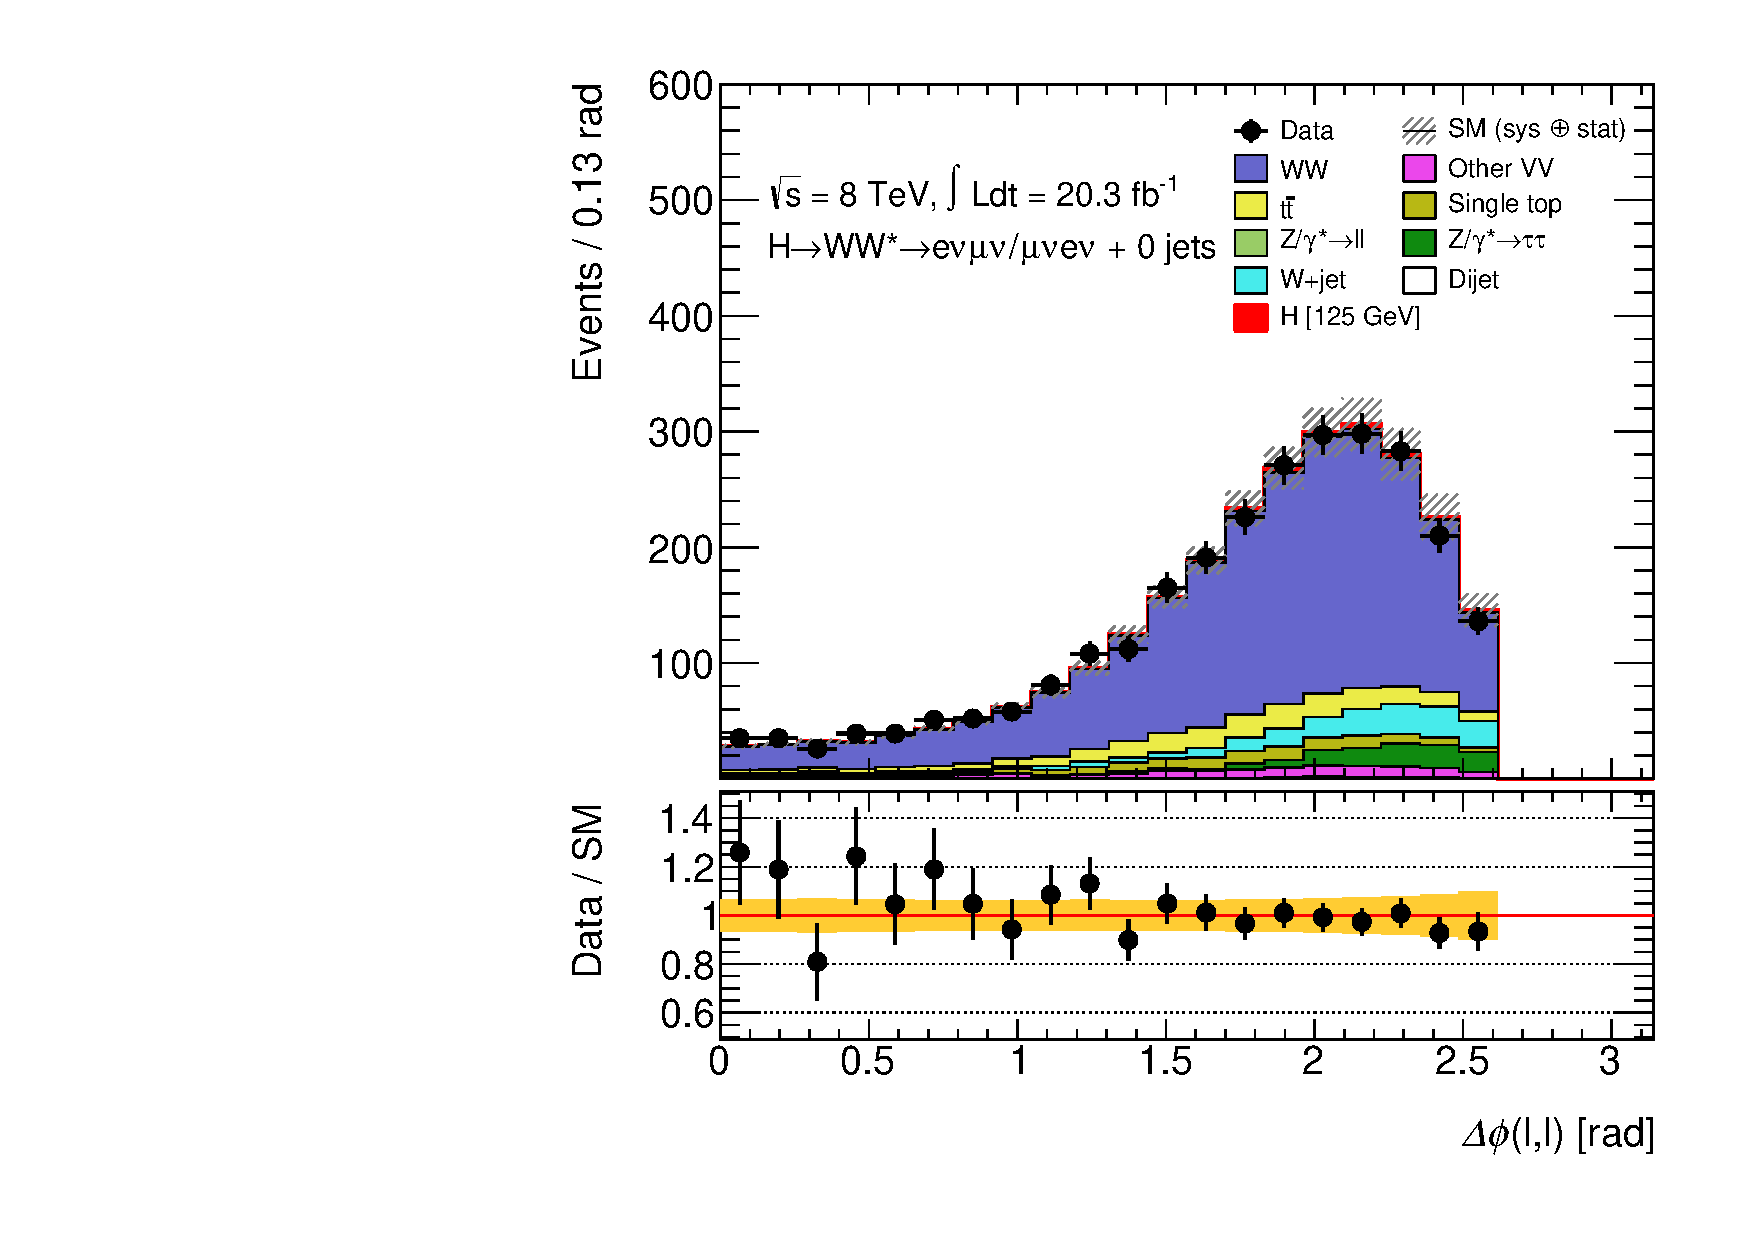
\includegraphics[width=0.495\textwidth]{tex/ww/emme_CutWWControl_0jet_DPhill_mh125_lin}
	\hfill
	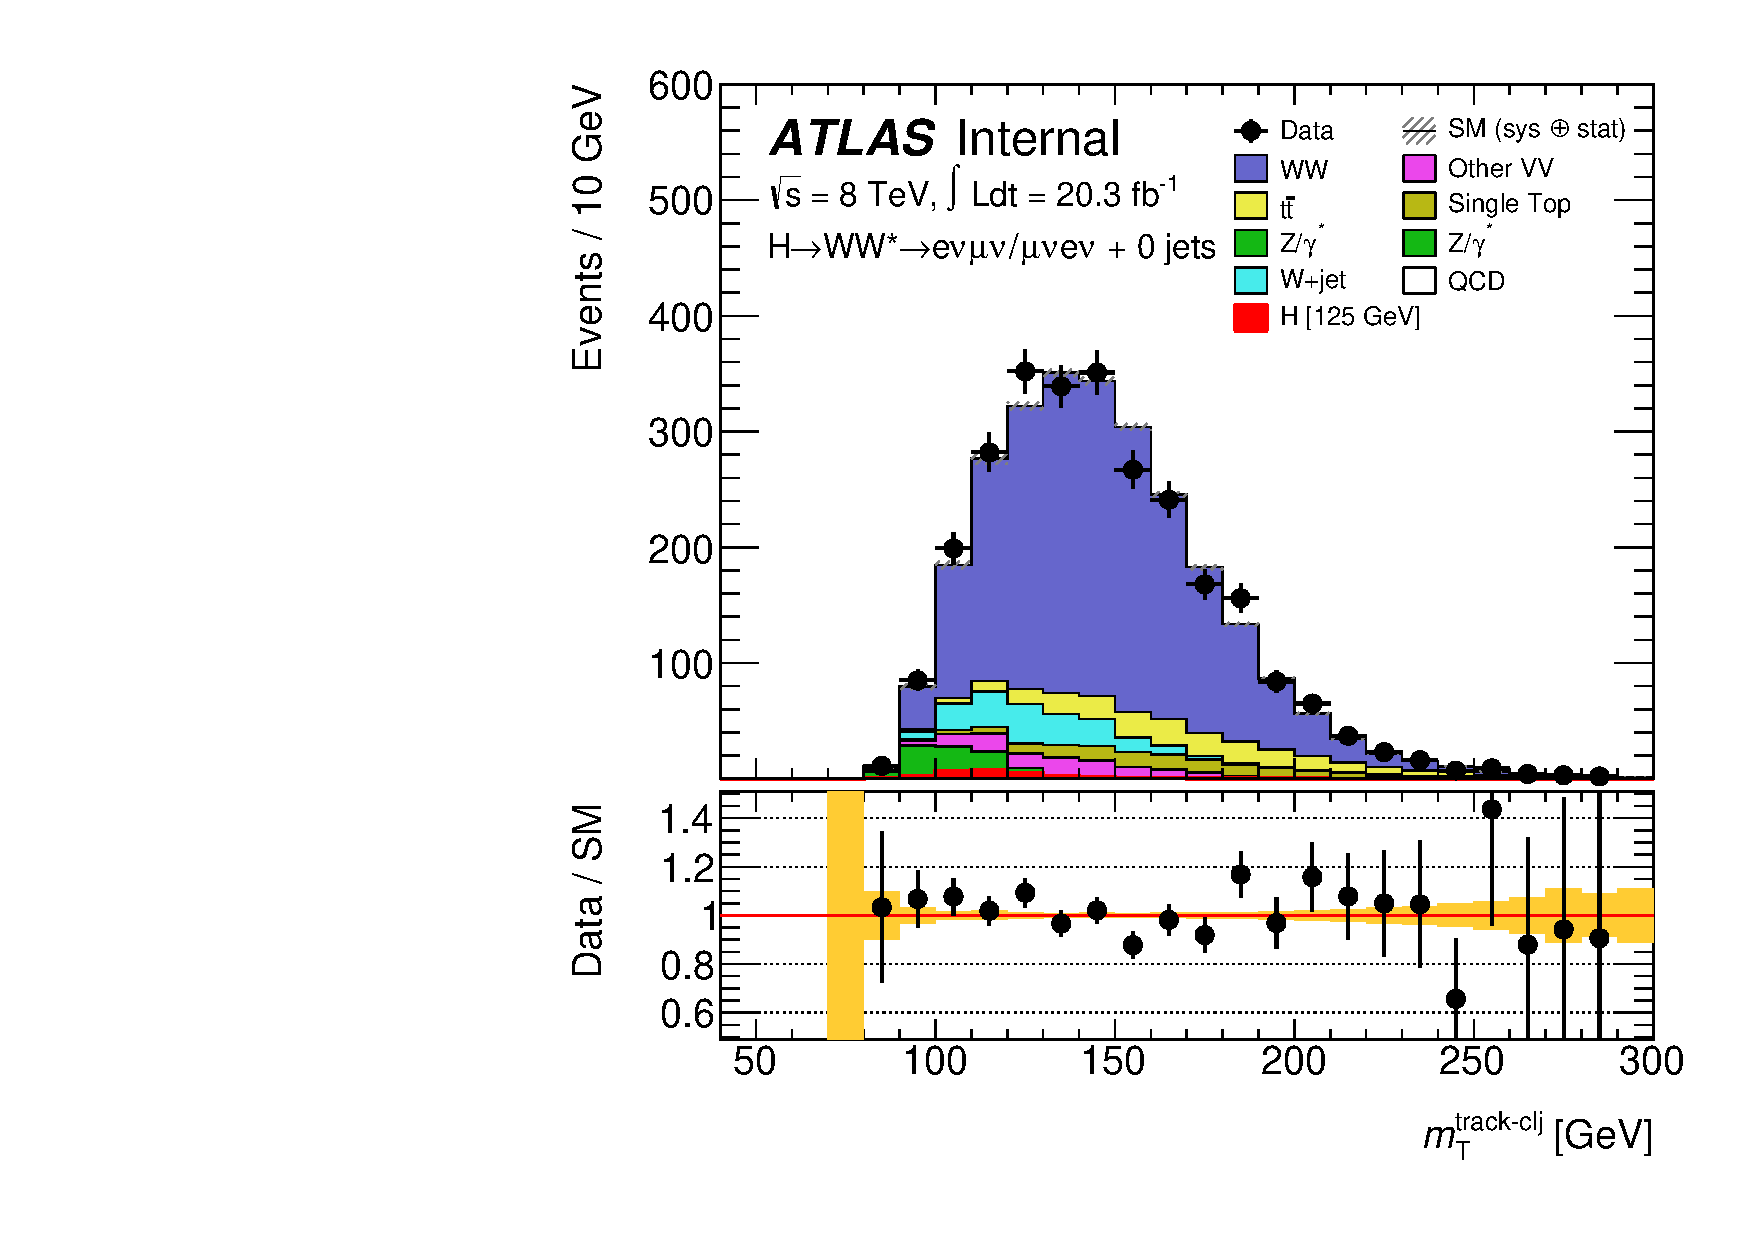
\includegraphics[width=0.495\textwidth]{tex/ww/emme_CutWWControl_0jet_MT_TrackHWW_Clj_mh125_lin}
	\\
	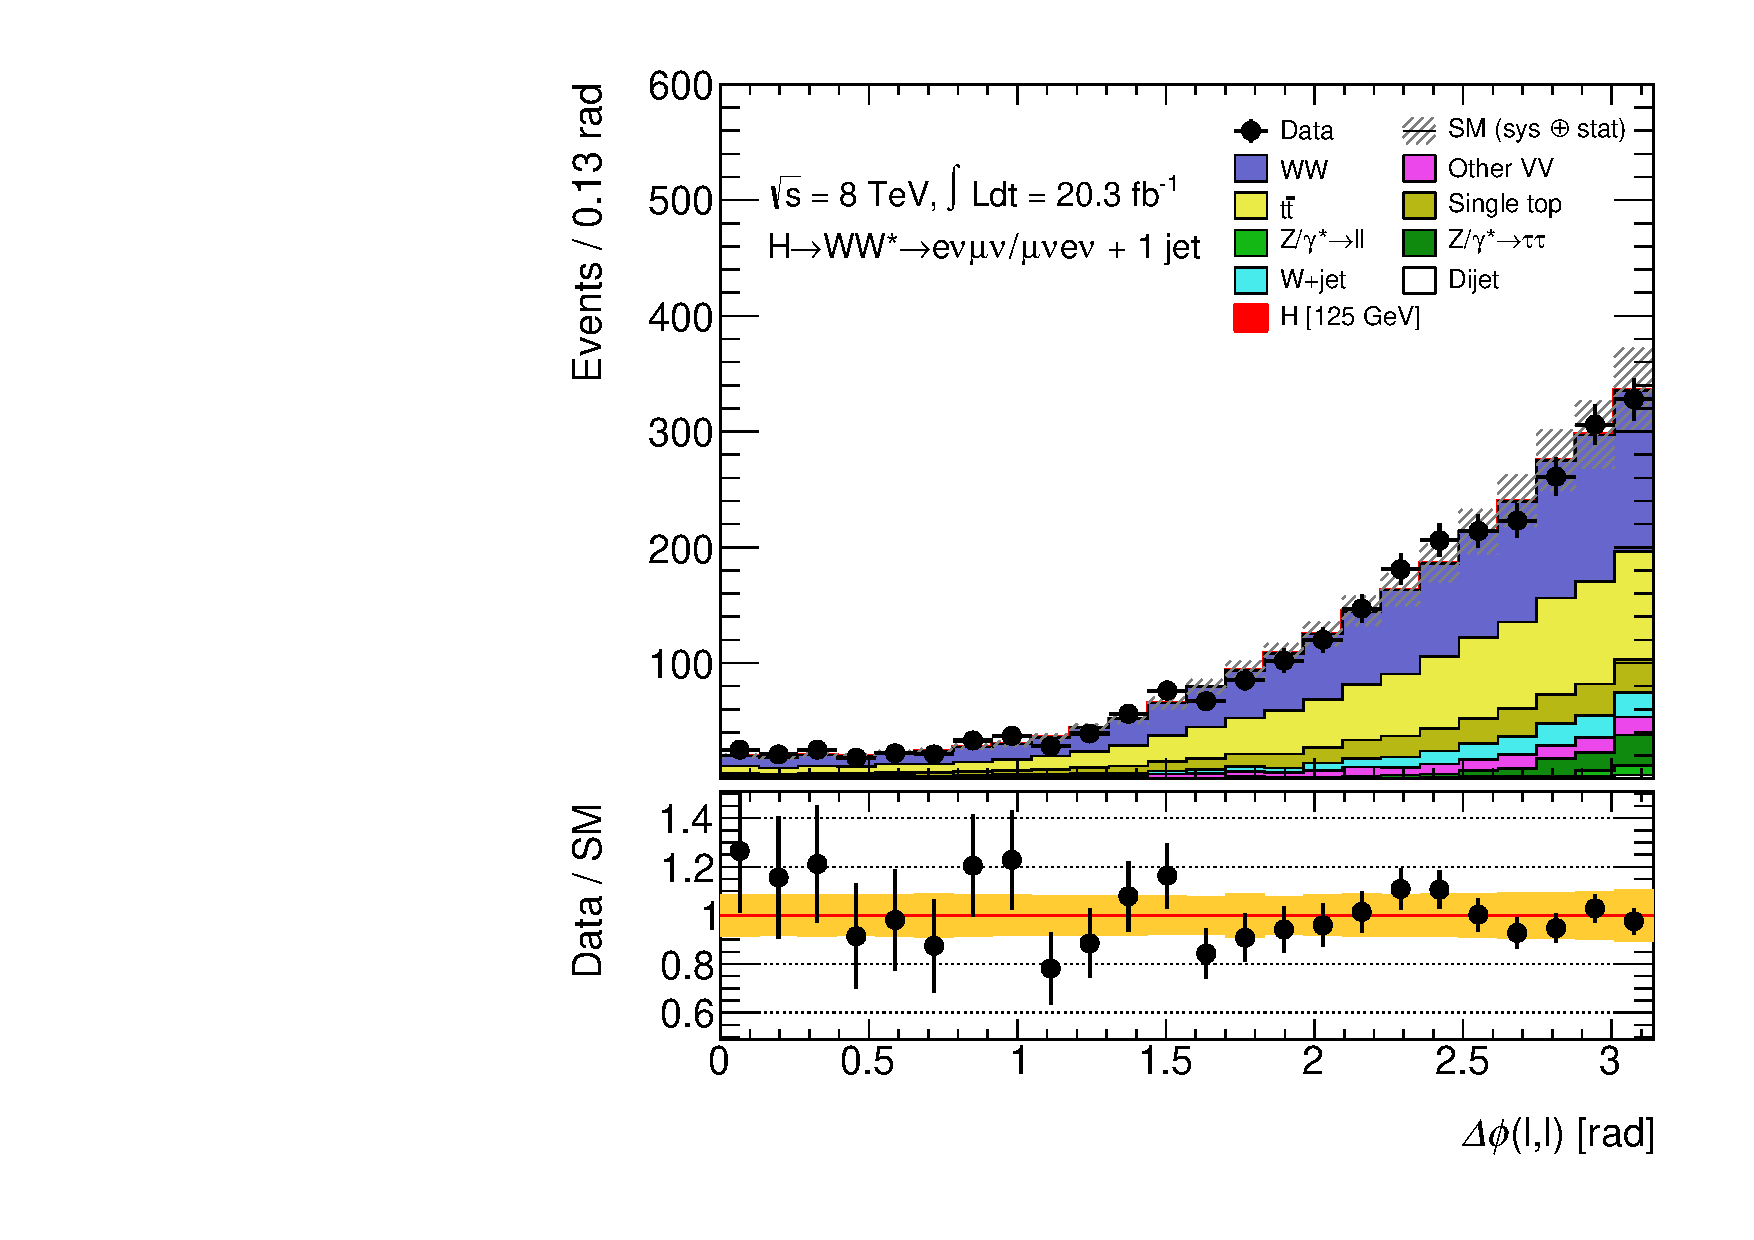
\includegraphics[width=0.495\textwidth]{tex/ww/emme_CutWWControl_1jet_DPhill_mh125_lin}
	\hfill
	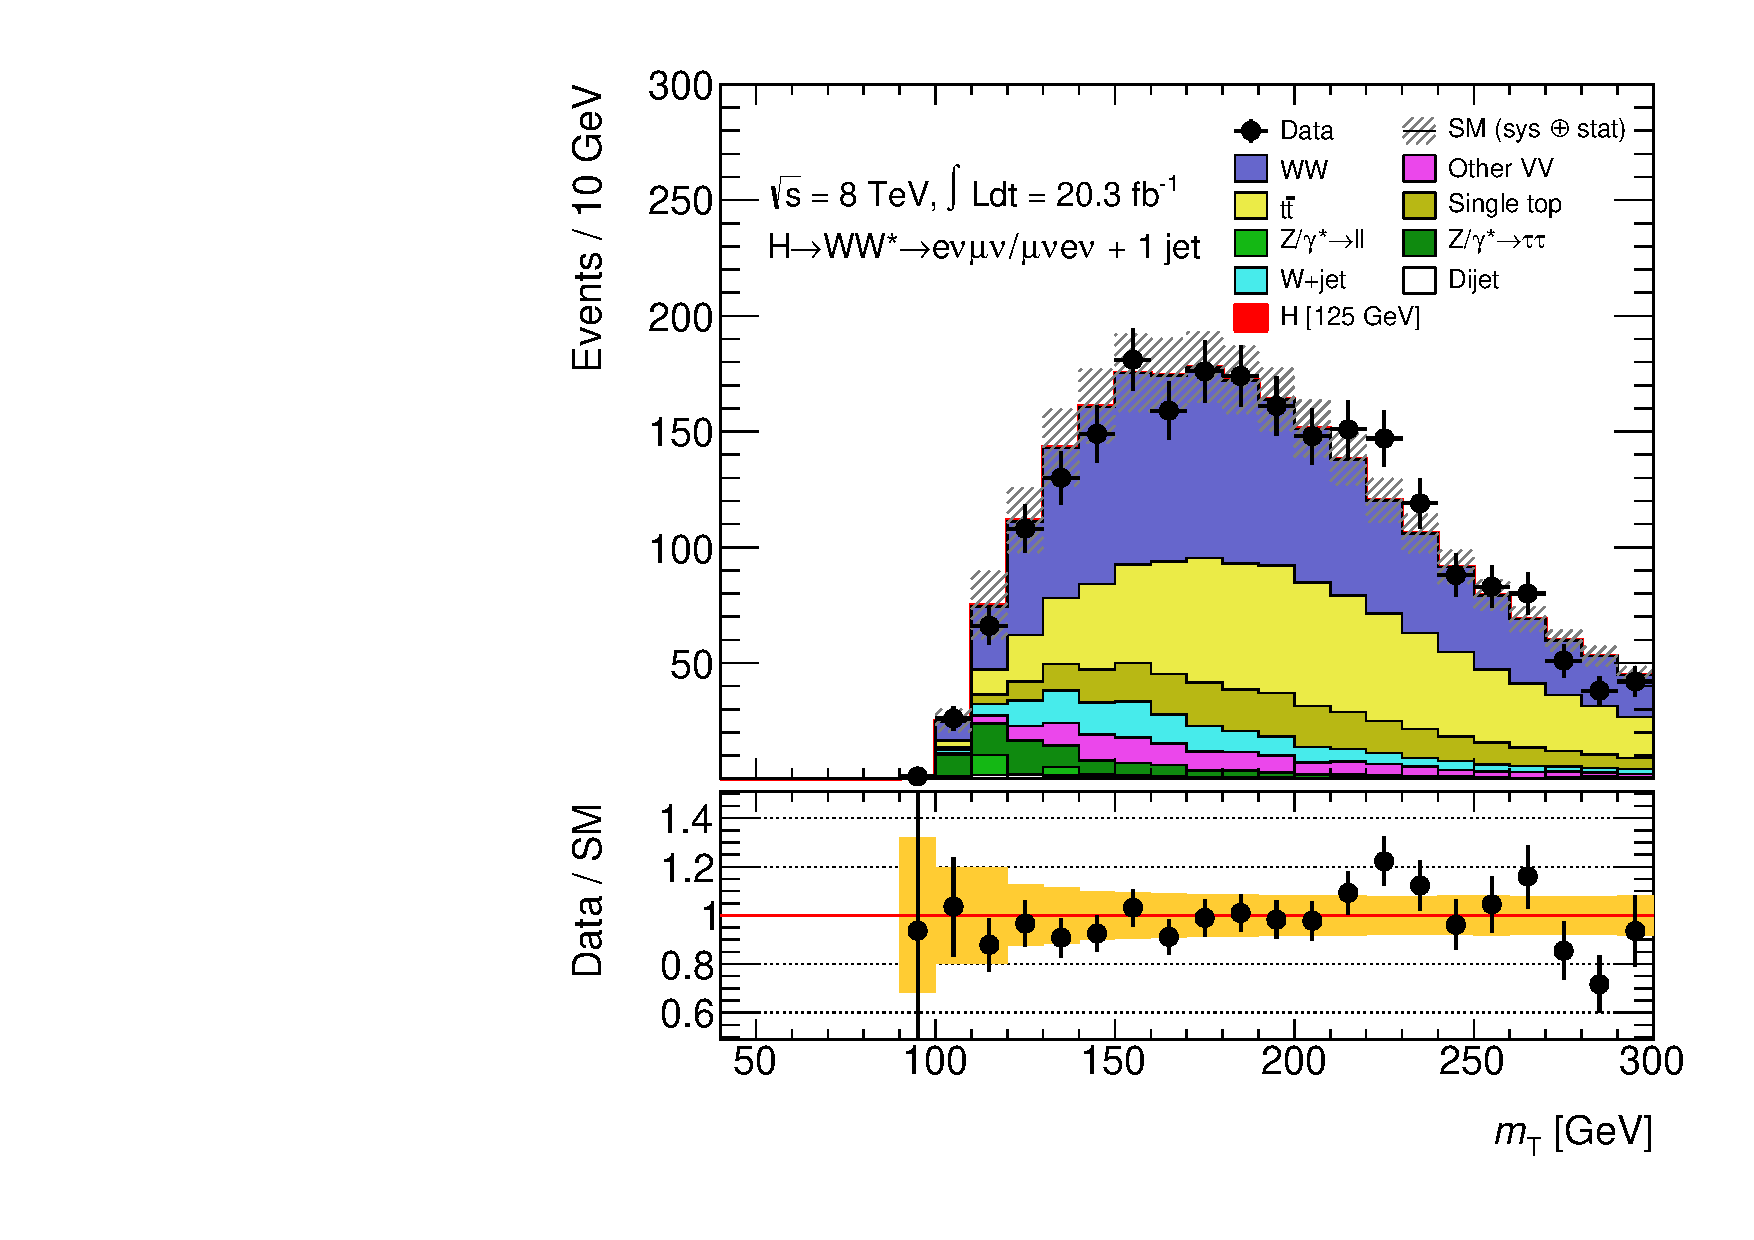
\includegraphics[width=0.495\textwidth]{tex/ww/emme_CutWWControl_1jet_MT_TrackHWW_Clj_mh125_lin}
	\caption{The \dphill (left) and \mt (right) distributions in the \WW control regions 
	of the 0-jet (top) and 1-jet (bottom) bins. Normalisation factors have been applied.}
	\label{fig:ww_bkg:cr_plots}
\end{figure}


\subsection{Theoretical uncertainties in $\alpha_{\WW}$}
\label{sec:ww_bkg:alpha}

Theoretical uncertainties in the extrapolation parameters $\alpha_{\WW}$ are evaluated 
at hadron-level (\ie before detector simulation) by changing some aspect of the MC 
modelling and measuring the effect upon each $\alpha_{\WW}$. This is done using NLO \WW 
MC. Uncertainties due to \ggWW diagrams are negligible, since these diagrams only 
contribute \about5\% (\about7\%) to the 0-jet (1-jet) bin SRs.

The event selection criteria used in evaluating the uncertainties is similar to the 
detector-level selection of the signal regions (see \Table~\ref{tab:event_selection}) 
and control regions (see \Table~\ref{tab:ww_cr_sel}). However, the \Pbottom-jet veto and 
\frecoil cuts are omitted.

Hadron-level object definitions follow. The MC event record is used to identify leptons 
and neutrinos which descend from the \PW bosons. An \metvec vector is constructed from 
the neutrinos. Each lepton is `dressed' with the four-momenta of photons within a cone of 
$\Delta R < 0.1$, in order to recover energy lost via QED FSR. Jets are found using 
individual particles as inputs (\cf topo-clusters at detector-level). Muons and neutrinos 
are excluded from jet finding since they interact weakly with the calorimeter. Objects 
must pass the same \pt, $\eta$ and overlap removal criteria applied at detector-level.

Four sources of theoretical uncertainty are considered:
\begin{itemize}[noitemsep,nolistsep]
	\item higher order corrections,
	\item PDFs,
	\item parton shower, hadronisation and underlying event models,
	\item NLO-PS matching scheme.
\end{itemize}

Uncertainties due to higher order corrections are evaluated via independent variation of 
renormalisation and factorisation scales in the range $\mu_0/2 \leq \mur,\muf 
\leq 2\mu_0$, where $\mu_0 = m_{\WW}$ is the nominal scale, whilst observing the 
constraint $1/2 \leq \mur/\muf \leq 2$. These are evaluated with \amcatnlo and validated 
with \mcfm.

Uncertainties due to PDFs are evaluated in two ways. Predictions with the MSTW 2008 
\cite{MSTW} and NNPDF 2.3 \cite{NNPDF} PDF sets are compared to those with the CT10 
\cite{CTEQ} PDF sets, and the maximum deviation is found. Also, the set of PDF 
eigenvectors corresponding to 90\% CL of the CT10 fit were used to evaluate an 
uncertainty, which was then rescaled to 68\% CL. These are evaluated using \amcatnlo.

Uncertainties due to the PS, hadronisation and UE models are evaluated by 
comparing \powhegbox showered by \pythia{6} (nominal) and \fherwig. 
Uncertainties due to the NLO-PS matching scheme are evaluated by comparing 
\meps{\powhegbox}{\fherwig} to \meps{\amcatnlo}{\fherwig}.

The $\alpha_{\WW}$ uncertainties for each signal region used in the fitting procedure are 
shown in \Table~\ref{tab:ww_bkg:alpha_unc}. Those for the validation region are shown 
additionally.

\begin{table}
	\centering
	\begin{tabular}{ccc|ccccc}
		\toprule
		& \mll & \ptsubleadlep & \multirow{2}{*}{Scale} & \multicolumn{2}{c}{PDF} & \multirow{2}{*}{PS/UE} & \multirow{2}{*}{NLO-PS} \\
		& (\GeV) & (\GeV) & & collab. & 68\% CL & & \\
		\midrule
		\multicolumn{8}{c}{\eech/\mmch channels} \\
		\midrule
		0-jet & 12--55 & $>10$ & 0.8\% & 0.5\% & 1.0\% & $-1.2\%$ & $+2.4\%$ \\
		1-jet & 12--55 & $>10$ & 0.8\% & 0.5\% & 0.7\% & $-2.3\%$ & $+3.8\%$ \\
		\midrule
		\multicolumn{8}{c}{\emch/\mech channels} \\
		\midrule
		\multirow{6}{*}{0-jet}
		& \multirow{3}{*}{10--30}
	    &  10--15 & 0.7\% & 0.9\% & 0.2\% & $+2.2\%$ & $+0.4\%$ \\
		&& 15--20 & 1.2\% & 0.8\% & 0.2\% & $+1.7\%$ & $+0.9\%$ \\
		&&  $>20$ & 0.7\% & 0.5\% & 0.3\% & $-1.9\%$ & $+3.1\%$ \\
		\cmidrule(lr){2-8}
		& \multirow{3}{*}{30--55}
		&  10--15 & 0.7\% & 0.8\% & 0.1\% & $+1.5\%$ & $+0.5\%$ \\
		&& 15--20 & 0.8\% & 0.7\% & 0.2\% & $+1.0\%$ & $+1.0\%$ \\
		&&  $>20$ & 0.8\% & 0.4\% & 0.5\% & $-2.4\%$ & $+3.9\%$ \\
		\cmidrule(lr){1-8}
		\multirow{6}{*}{1-jet}
		& \multirow{3}{*}{10--30}
	    &  10--15 & 3.1\% & 0.5\% & 0.1\% & $-2.4\%$ & $-3.4\%$ \\
		&& 15--20 & 1.6\% & 0.5\% & 0.1\% & $-3.0\%$ & $+0.7\%$ \\
		&&  $>20$ & 1.0\% & 0.6\% & 0.2\% & $-3.6\%$ & $+5.3\%$ \\
		\cmidrule(lr){2-8}
		& \multirow{3}{*}{30--55}
		&  10--15 & 3.2\% & 0.5\% & 0.1\% & $-2.0\%$ & $+1.9\%$ \\
		&& 15--20 & 1.5\% & 0.4\% & 0.1\% & $-3.0\%$ & $+2.4\%$ \\
		&&  $>20$ & 1.3\% & 0.5\% & 0.4\% & $-3.1\%$ & $+5.6\%$ \\
		\midrule
		\multicolumn{8}{c}{Validation region (\emch/\mech channels)} \\
		\midrule
		0-jet & $>110$ & $>15$ & 0.6\% & 0.6\% & 2.0\% & $+4.3\%$ & $-5.1\%$ \\
		\bottomrule
	\end{tabular}
	\caption{Theoretical uncertainties in the \WW extrapolation parameter $\alpha_{\WW}$ 
	for each signal region used in the fitting procedure, and also for the validation 
	region.}
	\label{tab:ww_bkg:alpha_unc}
\end{table}



\subsection{\mt shape modelling}
\label{sec:ww_bkg:mt}

Theoretical uncertainties in the shape of the \mt distribution are also investigated, 
as they could affect the fit. Uncertainties due to scale, PS/UE and NLO-PS choices are 
considered within each signal region separately, using the methods described above.

Each uncertainty is parametrised by fitting the ratio of the \mt shapes, and then 
symmetrising the fit to produce ``up'' and ``down'' variations. The \mt distributions are 
normalised to unit integral in order to remove effects from acceptance uncertainties. 
In cases where multiple variations exist within a single uncertainty source (such as the 
seven scale variations), the largest deviation from the nominal result is fit. A linear 
fit is used in the central \mt region, and a constant is used in the low-\mt and 
high-\mt tails of the distribution where statistical fluctuations dominate.

These fits allow the hadron-level \mt distribution of the \WW background to be reweighted 
to the ``up'' and ``down'' variations. In this way, the \mt shape uncertainty is treated 
as a nuisance parameter in the \HWW fitting procedure. The uncertainties for the 0-jet 
and 1-jet signal regions are displayed in Figures~\ref{fig:ww_bkg:mTshape_0j} and 
\ref{fig:ww_bkg:mTshape_1j} respectively, and additionally a global fit is shown.

\begin{figure}
	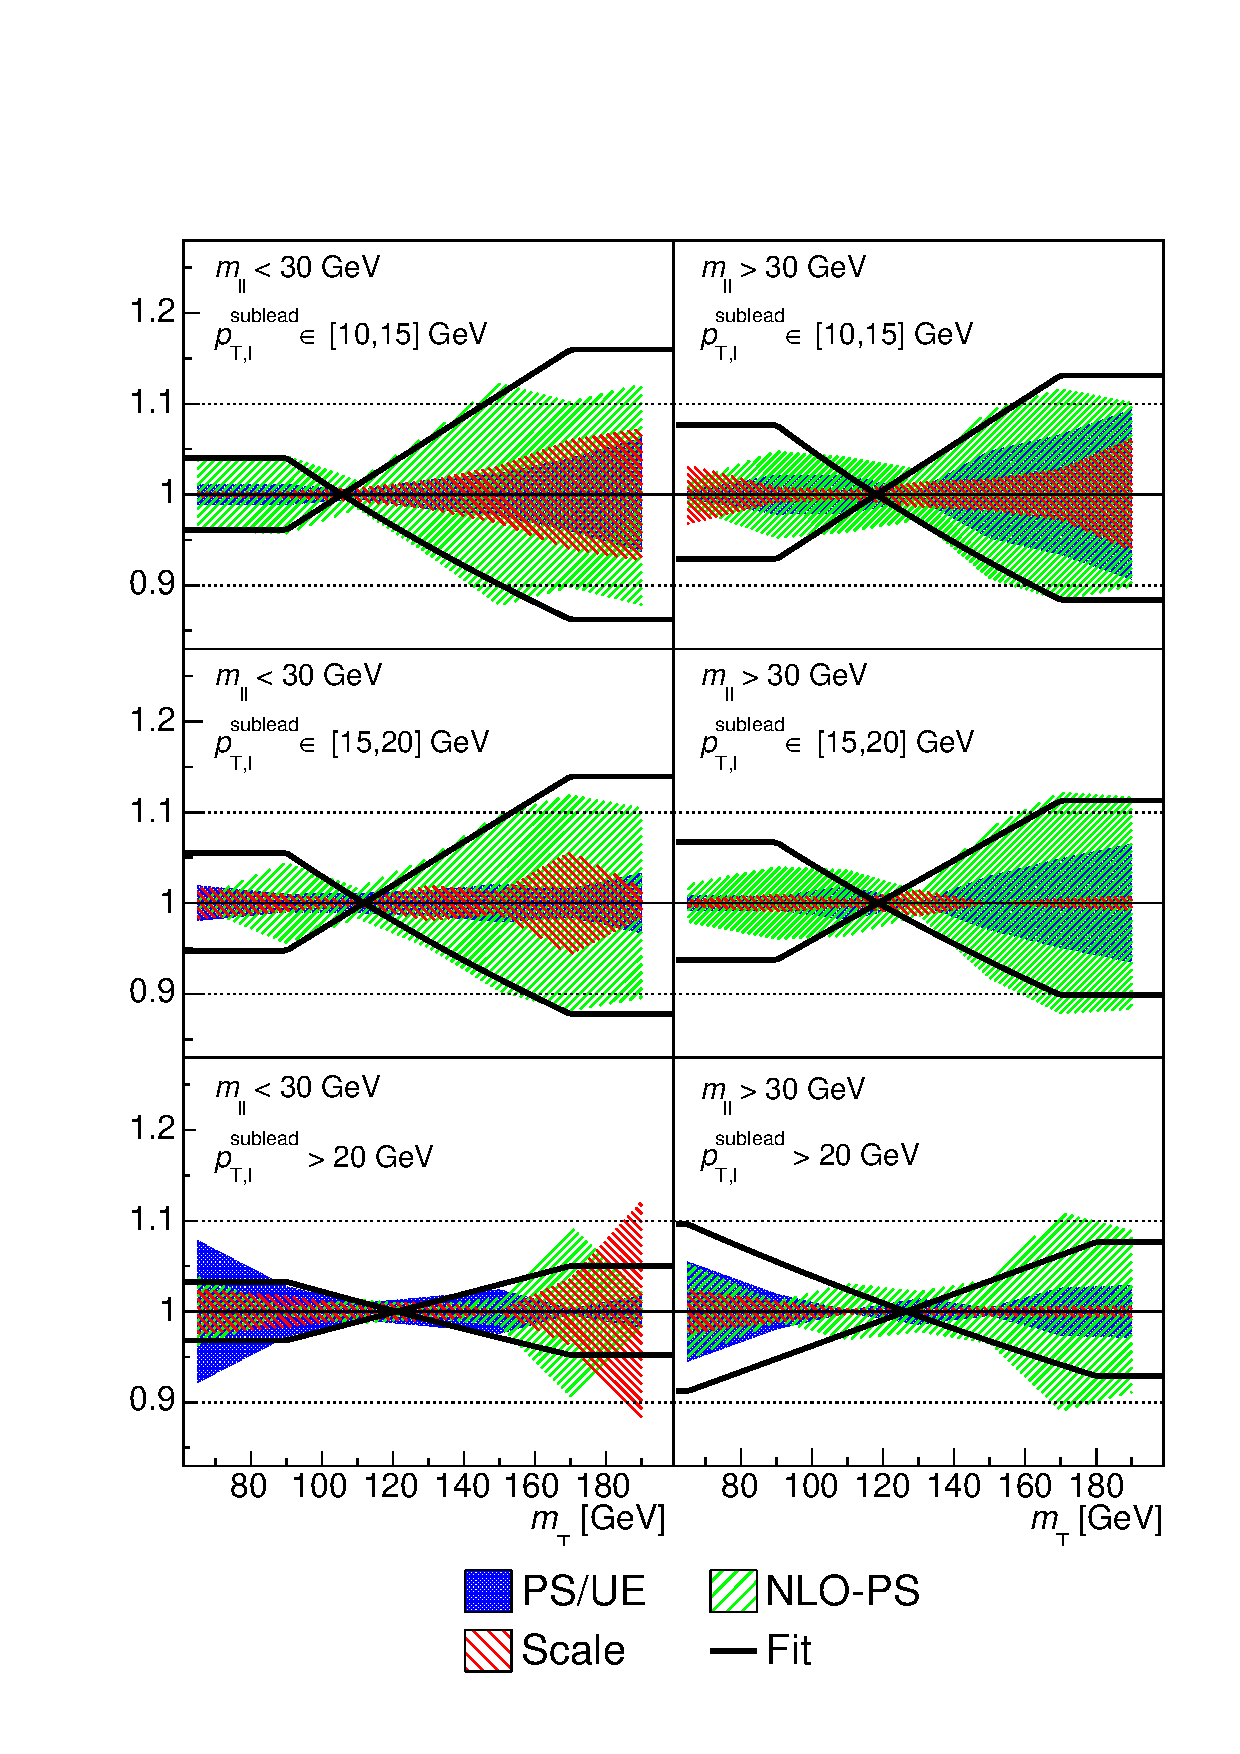
\includegraphics[width=\hugefigwidth]{tex/ww/mTshape_df_0j}
	\caption{\WW \mt shape systematic uncertainties in each 0-jet signal region for the 
	\emch/\mech channels. The fit shown is the sum in quadrature of the three individual 
	fits, and successfully envelopes the uncertainty sources.}
	\label{fig:ww_bkg:mTshape_0j}
\end{figure}

\begin{figure}
	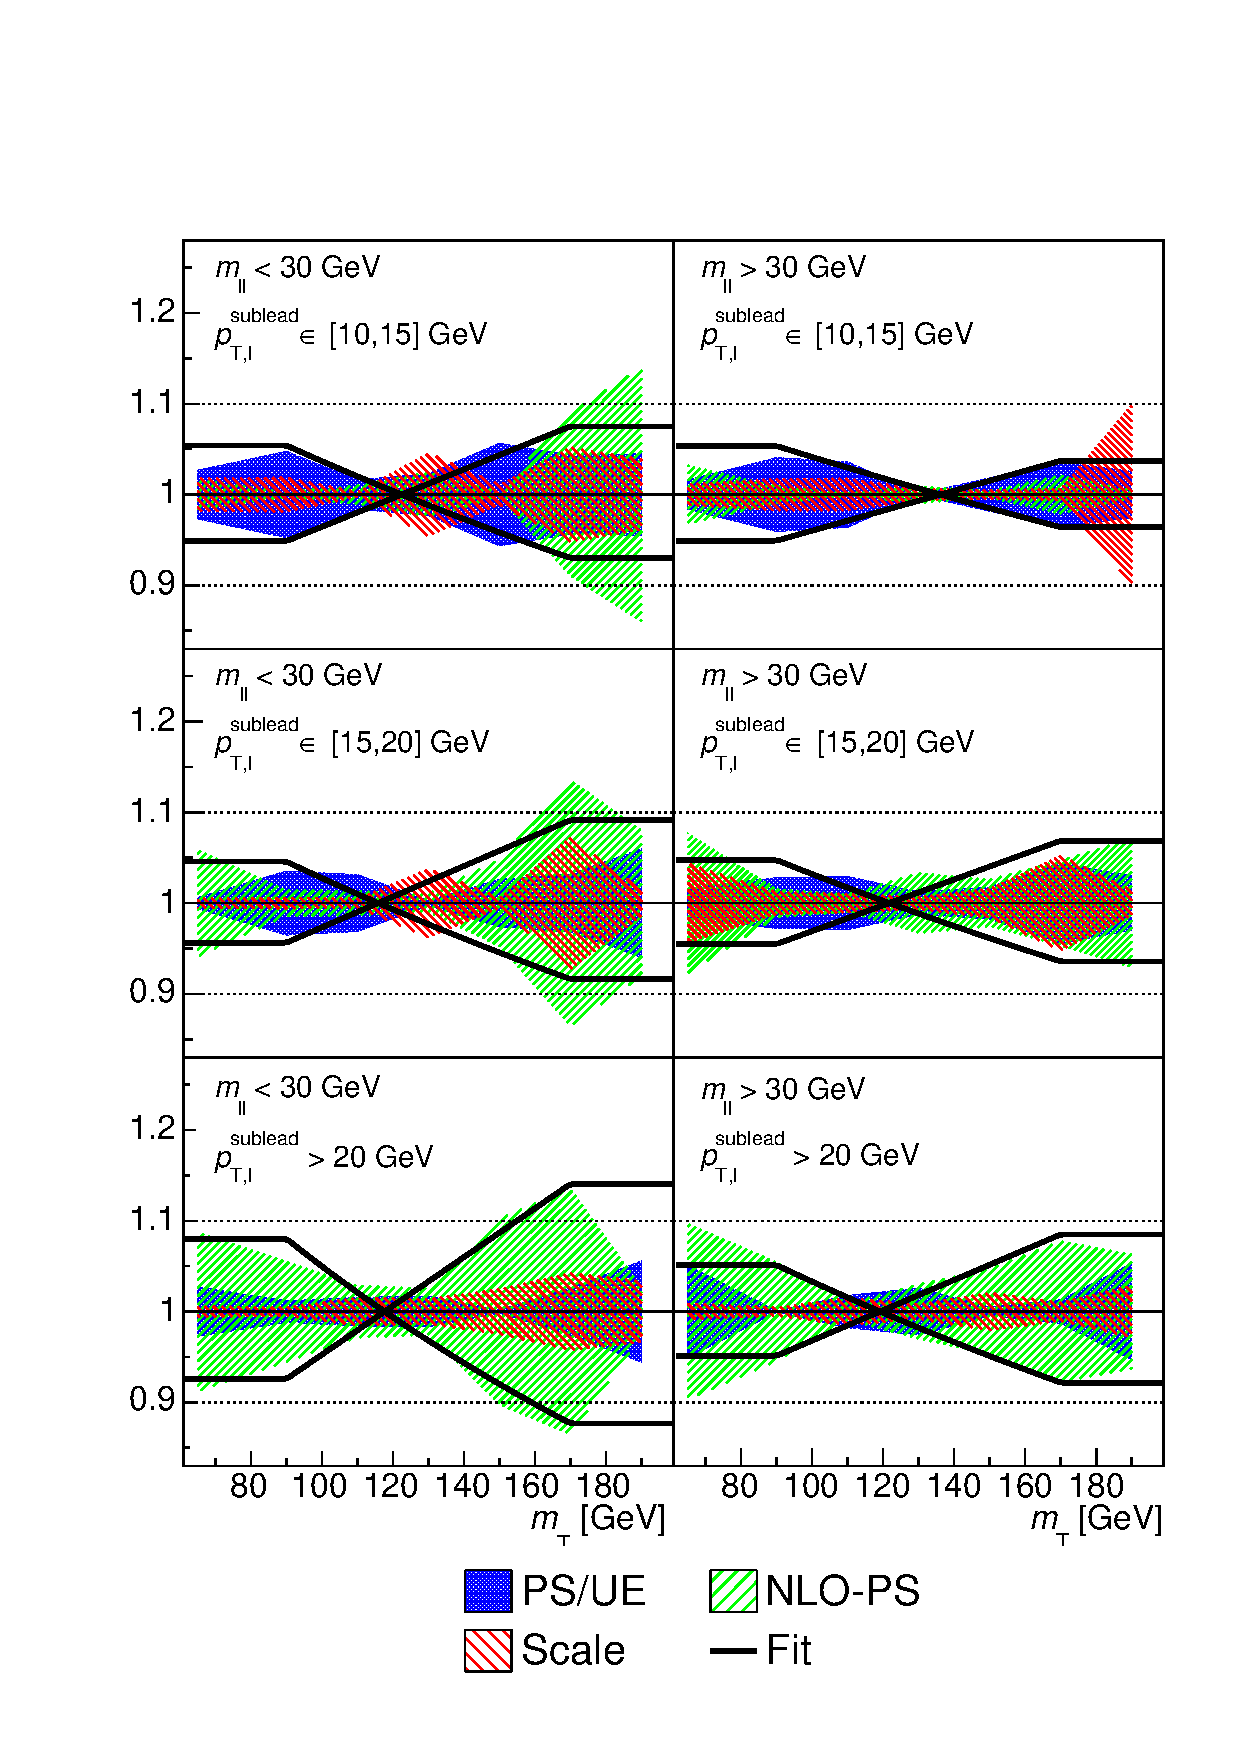
\includegraphics[width=\hugefigwidth]{tex/ww/mTshape_df_1j}
	\caption{\WW \mt shape systematic uncertainties in each 1-jet signal region for the 
	\emch/\mech channels. The fit shown is the sum in quadrature of the three individual 
	fits, and successfully envelopes the uncertainty sources.}
	\label{fig:ww_bkg:mTshape_1j}
\end{figure}



\subsection{\WW background in the \twojet bin}
\label{sec:ww_bkg:2j}

In the \twojet bin the \WW background is modelled by \sherpa, since the second jet 
is described by the parton shower in \meps{\powhegbox}{\pythia{6}}. Two kinds of diagrams 
can be identified for the \WW~+~2~jets process: electroweak production (with zero QCD 
vertices at LO) and QCD production (with two QCD vertices at LO), where VBF \WW 
production is included in the former. 

The two production types are simulated separately at LO by \sherpa, and this causes their 
interference to be neglected. Interference with VBF Higgs boson production diagrams is 
also neglected. The effect of each interference is investigated and treated as a 
systematic uncertainty.

\todo[inline]{Come back to WW+2j background}
\todo[inline]{Validation region is validated?}
